\documentclass{article}
\usepackage[letterpaper, margin=2cm]{geometry}
\usepackage{amsmath,graphicx}
\usepackage{multicol}
\usepackage[font=scriptsize,labelfont=bf]{caption}
\usepackage{sectsty}

\sectionfont{\fontsize{12}{15}\selectfont}
\captionsetup{width=\textwidth}
\graphicspath{./}

\title{Hydroelectric Turbine PID Speed Governor}
\author{
    Anderson, Colin
    \and
    Potter, Kalen
    \and
    Tsosie, Naakaii
    \and
    VanShaar, Janson
}
\date{}


\begin{document}
    \maketitle

    \thispagestyle{plain}
    
    \noindent\makebox[\linewidth]{\rule{\textwidth}{0.4pt}}

    \begin{center}
        \textbf{Abstract}
    \end{center}


    A project exploring the real scenario of the Sayano-Shushenskaya power station 
    accident that occurred in 2009.  A simulated model of a single power generation 
    system at the site is developed.  The model shows how the opening of the water flow 
    gate is changed through a typical year to reach maximum power generation without 
    damaging the turbine.  The model is then fitted with a First Order Plus Dead Time 
    (FOPDT) model to generate controller parameters for a PID controller that automates 
    the opening and closing of the watergate.  Implications, environmental factors, 
    and public safety of using the system is also discussed.

    \noindent\makebox[\linewidth]{\rule{\textwidth}{0.4pt}}

    \begin{multicols*}{2}
        \newlength{\mywidth}
        \setlength{\mywidth}{\linewidth}
        \addtolength{\mywidth}{-0.5\columnsep}

        \section{Introduction}

        In 2009, the Sayano-Shushenskaya power station in Russia failed catastrophically.  The cause of failure was determined to be from operating the power station under conditions that caused excess vibrations. These vibrations caused major wear and tear to the system, and before maintenance procedures found this, the turbine materials failed and exploded, damaging the surrounding structures.  This power station is restricted to operate between bands of 0-350 MW and 550-650 MW. If the outputs are not within these bands, the generators physically shake and shorten their mechanical lifespan.  For this reason, transition between the bands must also be quick. Because the station has a set point of power output, our objective is to design and code a PID controller to manage the valve that controls the input flow. 

        \section{Progress Report \#1}

        We are modeling a turbine power generation system, with a desire to maintain the power output within certain “safety zones” in order to reduce vibrations on the generator. We control the power output of the system by adjusting the dam gate valve in order to let water flow through. Thus, the input for our process is our valve position, which controls the gate height, and the output is the power produced by the turbine. These two variables are related through a series of equations. The first is: 

        \begin{equation}
            q=A\sqrt{2gh}
        \end{equation}

        which calculates our flow (q) based on the height of the water in relation to the turbine entrance (h), and the area of the gate that is available for water to flow through (A). In this situation, h is a variable because the dam level will change seasonally throughout the year, and A will fluctuate with our input. g is the gravitational acceleration constant (9.8 m/s2). We then plug that equation into our overall energy balance:

        \begin{equation}
            W=\eta \rho gA\sqrt{2gh}\Delta z
        \end{equation}

        where $W$ is our power output, $\eta$ is our turbine efficiency (which is a constant at $0.8286$), $\Delta z$ is the height of the gate, and $\rho$ is the density of water (assumed to be constant at $998.29\ kg/m^3$). Our process will be automatically adjusting the valve position to account for the dam level, in order to keep the power output within acceptable ranges.

        The current literature outlines the problem and experimental solutions used at the time. The “2009 accident update”1  gives a detailed look at the background and the “Hydro-turbine governor control: theory, techniques and limitations”2 outlines PID controller and theories used in power plants.

        \section{Progress Report \#2}

        Due to the nature of the subject, we opted for simulated data and responses.  In order to ultimately design a control system, some starting parameters must be derived using an FOPDT model.  We quickly found out that our system is nonlinear when we have the conditional statements when the system transitions from high power to low power operating zone, making it difficult to construct an FOPDT model because the gain changes if we view it like that.  We also noticed the height ends up being squared so it doesn’t behave as linearly.  Our solution was to act as though the power output is actually our set point, the dam level is placed as just some intermediate internal calculations, and the output is the height. This resulted in the data displayed below, where our process variables are $K_p = 1.0$, $\tau_p = 1.8\ days$, and $\theta_p = 0.0\ days$.

        
        \vspace{5mm}
        \noindent
        \begin{minipage}{0.49\textwidth}
            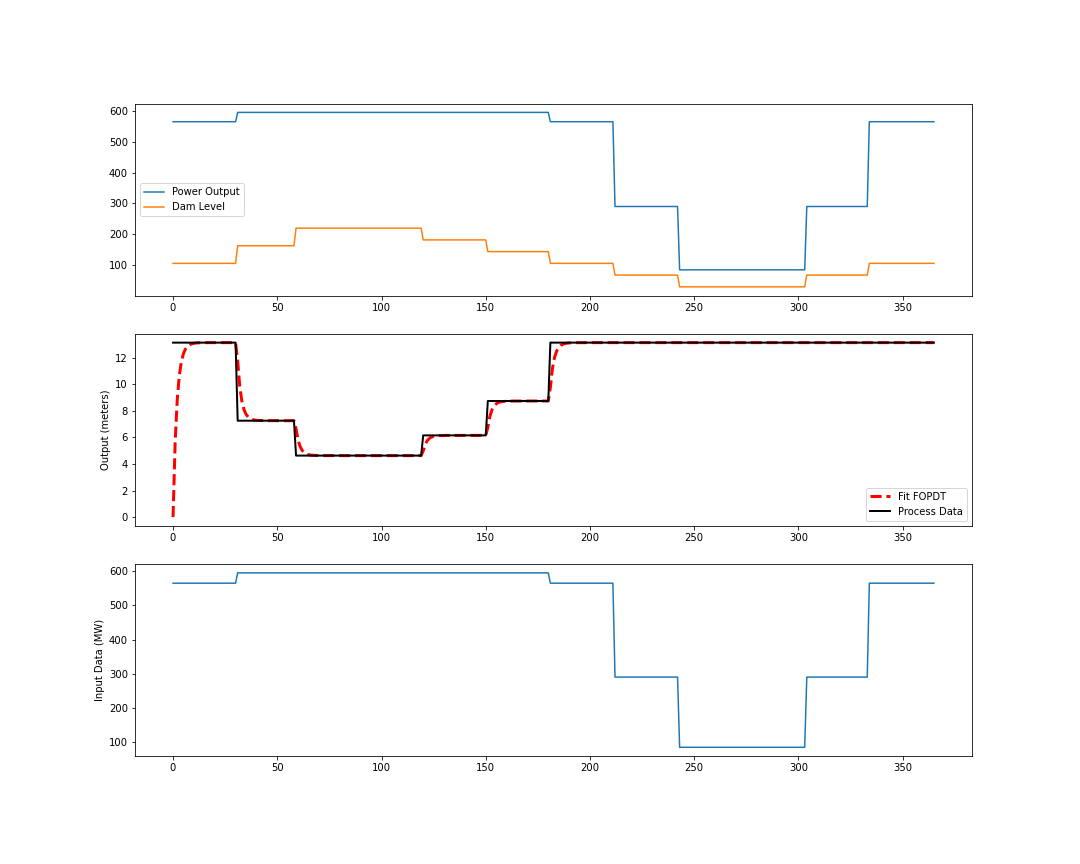
\includegraphics[width=\textwidth]{FOPDT.png}
            \captionof{figure}{FOPDT Model Fit}
        \end{minipage}
            
        \section{Progress Report \#3}
    
        A PID controller can now be constructed using the parameters determined previously.  While tuning, we had to reduce the gain (Kp) by 25\%, because of oscillations that occurred and caused the system to occasionally spend excess time outside the safety zone in more areas than the large jump at t = 212 days.  As mentioned earlier, it is important to reduce the oscillations or excessive wear and tear that may occur and cause catastrophic failure.

        Occasionally the systems need to be serviced and turned off.  Due to the limitations of the controller, initial startup of the system and changing from high to low power will require manual adjustment; otherwise the system will be operating outside the safety zones for a whole week, where it can be damaged severely.  Once the adjustments are made, then the controller can be reactivated for safe automated operation.

        \vspace{5mm}
        \noindent
        \begin{minipage}{0.49\textwidth}
            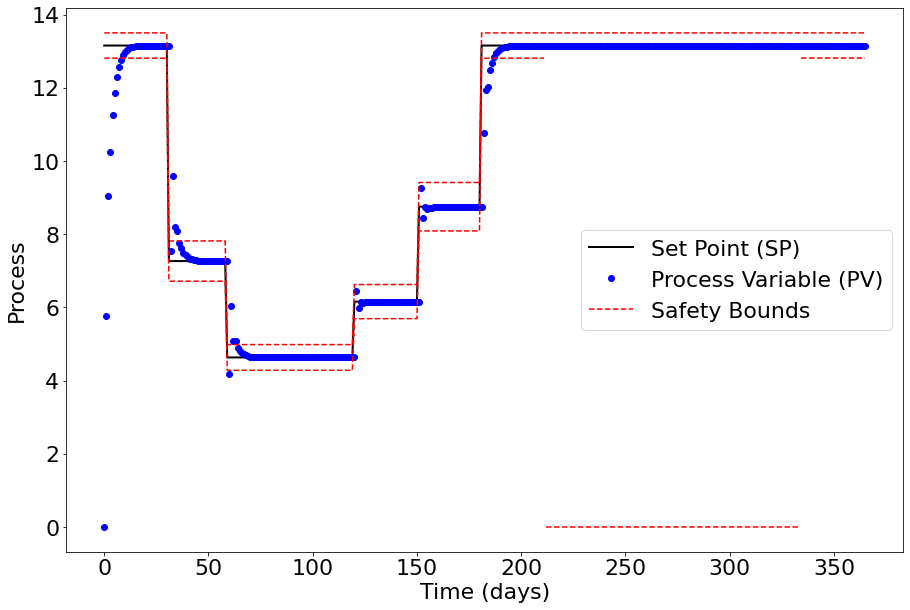
\includegraphics[width=\textwidth]{projectPID_untuned.png}
            \captionof{figure}{Untuned PID Controller}
        \end{minipage}

        \noindent
        \begin{minipage}{0.49\textwidth}
            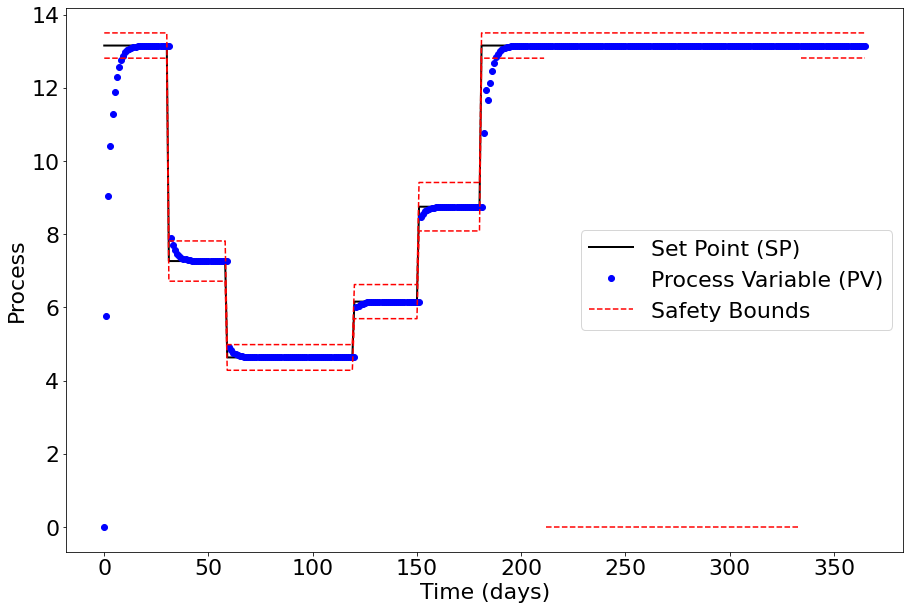
\includegraphics[width=\textwidth]{projectPID_tuned.png}
            \captionof{figure}{Tuned PID Controller}
        \end{minipage}

        \section{Non-Technical Considerations}

        Turbine speed governors are a critical part of a hydroelectric power plant, and failure has catastrophic consequences. The 2009 accident at the Sayano-Shushenskaya power plant killed 75 people and led to widespread power outages. Therefore, it is important to not only consider the impact of the control system, but the impact of the dam and hydroelectric power plant.

        The construction of a dam is a massive project that has consequences for those living in the area. Changes to water flow and the creation of a reservoir can negatively impact local wildlife as well as displace local residents; such was the case with the construction of Bhakra Dam in northern India. 

        The generation of electricity impacts many aspects of life, including public welfare and the environment. The purpose of a hydraulic dam is to generate clean energy which protects the environment. Access to that energy provides people with a higher quality of life and greater economic opportunity.

        This research would also include emergency preparations in case the dam breaks and overflow preparations. Along with this research, cities that would be impacted by an accident at the dam would need to create emergency plans.

        When designing the turbine, to reduce environmental stress, we recommend using a filter before the entrance of the dam, so that aquatic life and debris do not enter the turbine. We also recommend doing research into the effects of the dam on wildlife and the heights of streams in surrounding areas. Emergency plans need to be created to account for if these filters fail. These filters also need to be cleaned and replaced often.
        There are many benefits that a hydroelectric power plant provides, and a good control system ensures that the plant remains operational.

        \section{Conclusion}

        In conclusion, we were able to design and code a PID controller to manage the valve that controls the input flow.  One major assumption made was that the properties of the water are constant.  Another assumption is that all work generated from the dam comes from potential energy.  A further study would need to be done to find the pressure drops and work along the gate head that would be lost, as well as develop a higher order model that would account for the gain changes that were mentioned. This is a simple start to designing and coding a fully automated system for the hydroelectric station.  Though this would not be the best to implement into a current system, it does model a basic outline of the dam PID controller. 


    \end{multicols*}

\end{document}